\documentclass{standalone}

\usepackage{amsmath,scalerel}
\usepackage{tikz}

\begin{document}
	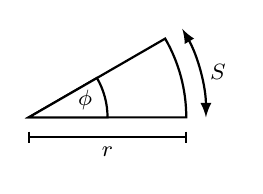
\begin{tikzpicture}
		[
		x=1cm, y=1cm, scale=1.0, font=\footnotesize, >=latex 
		%Voreinstellung für Pfeilspitzen
		]
		

		
		
		%Länge x Achse
		\draw [thick] (0,0) -- ++(2,0) node[below] {};
		\draw [thick] (1,0) node[below] {$r$};
		
		%Zahlen auf x-Achse
		\foreach \x in {0,2}
		\draw[shift={(\x,0)},color=black, thick] (0pt,2pt) -- (0pt,-2pt);
		
		%Winkelgugus
		\begin{scope}[xshift=0cm, yshift=0.25cm, rotate=0, scale=1]
			\filldraw[fill=white, thick] (0,0) -- (2,0) arc (0:30:2) -- cycle 
				node[midway, below, green!50!black, xshift=0pt, yshift=0pt] {};
			\filldraw[fill=white, thick] (0,0) -- (1,0) arc (0:30:1) -- cycle 
				node[midway, xshift=8pt, yshift=-1pt] {$\phi$};
		\end{scope}
		
		\draw [<->, thick] (2.25,0.25) arc (0:30:2.25) node[midway, right, xshift=0pt, yshift=0pt] {$S$};
	\end{tikzpicture}

\end{document}
